\chapter{Computational Intelligence and Machine Learning}
\label{Cap3}

In this chapter, the fundamentals of Computational Intelligence and Machine Learning 
are developed. Particularly, the focus of the chapter is to present the main tools 
used in this thesis, namely \emph{neural networks} and \emph{evolutionary algorithms}. To 
reach a general understanding of these tools, a brief description of learning mechanisms
and numerical optimization is carried out.

\section{Computational Intelligence}
The first thing to address is the meaning and scope of \emph{Computational 
Intelligence} (CI). With recent advancements in fundamental research in this area
and its sub-fields, there seems to be a blurry definition of what exactly is CI, and there 
is no concrete one until now. For this reason, in this work the definition of CI is an 
umbrella term for several other applications. However, these applications are related to 
each other for the same reason that CI exists: to provide a computational solution to a 
problem using as inspiration the paradigms of nature-inspired intelligence. For instance, 
following the handbook by Kacprzyk and 
Pedrycz~\cite{kacprzykSpringerHandbookComputational2015},
the definition of CI is to be a collection of nature-inspired computational methods that
provide solutions to problems where \emph{hard computing} is inefficient or it not even
suited to provide a solution to a given problem. Here, there is an important distinction
that should be carried throughout the remaining of the work: that there are problems for
which traditional tools are insufficient for the traditional problems. In this work, this
is the philosophy used to provide solutions: that the traditional methods might seem hard 
and unfitting to provide solutions to the problems presented, and therefore new ways of 
approaching these solutions should be used.

In general, CI methods do not provide exact and accurate results, but this is expected.
It does not mean that CI is providing the ultimate, best solution to a problem. Rather, it 
is providing an approximate solution that can be used later with more robust algorithms and
methods. CI is not meant to be used as the sole method to solve a problem, but instead to
help find \emph{some} solution to a difficult problem. That is why CI is considered an 
umbrella term, because it comprises diverse fields that can be used to find such an 
approximate solution. Indeed, in this work, two main field of CI are used:
\emph{neural networks}, which is a part of ML, a sub-field of CI; and
\emph{evolutionary algorithms}, which are stochastic optimization methods inspired by the 
evolution mechanisms found in nature.

\section{Machine Learning}
In modern times, data is constantly being created and used to model the reality around us.
However, traditional methods (hard computing) have not been enough to handle the large
data sets created. For this reason, new ways of dealing with this information are needed. 
Most importantly, the need for automated discovery and \emph{pattern recognition} within the
data. Following Murphy~\cite{murphyMachineLearningProbabilistic2012}, ML 
is defined as the set of techniques that can automatically detect patterns in data, and use 
these patterns to create new predictions, or to perform other kinds of decision making.
In other words, \emph{the data creates the ML algorithm}, not the other way around.
It is with data that ML methods work, however, these methods are essentially
\emph{function approximation} methods, which shall be discussed in a later section.
For now, a brief overview of the different kinds of ML tasks and problems will be presented,
focusing primarily on \emph{supervised learning}. Nonetheless, there exist other types
of learning, such as \emph{unsupervised learning}~\cite{goodfellowDeepLearning2016,hastieElementsStatisticalLearning2009} and \emph{reinforcement learning}~\cite{suttonReinforcementLearningSecond2018,kaelblingReinforcementLearningSurvey1996},
which are out of scope of this work, but remain an important part of modern ML theory.

\section{Supervised Learning}
The most common kind of ML methods is that of \emph{predictive} learning. For a set 
\(\mathcal{D}={ \{(\bm{x}_{i}, y_i)\} }_{i=1}^{N}$ with inputs $\bm{x}\)
and outputs $y$, the goal of \emph{supervised learning} is to learn a map between
inputs and outputs. Here, $\mathcal{D}$ is the so-called \emph{training set} and $N$
is the number of \emph{training samples}.

In most common cases, the inputs $\bm{x}$ are $D$-dimensional vectors that
represent information about something. For instance, the height and weight of a
person, or the evolution of the stock market throughout the years. 
The components of these vectors are referred to as \emph{features} or \emph{attributes}.
The general form of $\bm{x}$ is not defined, it can be anything from an image, a time 
series, sentences from a text, graphs, molecules, and so on.

In a similar fashion, the \emph{response} variables $y$ can be, in general, anything. 
However, there is a clear distinction given the forms that these variables can take. For 
instance, if the variable $y$ has \emph{categorical} values, the supervised learning task 
is considered a \emph{classification} problem. Categorical values come from a finite set of 
possible values, \(y_{i} \in \{1, \dots, C\}\), and might represent any type of discrete or 
nominal value. For example, it might represent the colors in a clothing line, the gender 
between people, and so on. On the other hand, if the values of $y$ are real-valued, such 
that \(y_{i} \in \mathbb{R}\), then the learning task is dubbed a \emph{regression} problem.

\subsection{Classification}
In this section, the problem of classification is looked at with more detail. Although 
classification is not used at all in this thesis, it is helpful to discuss it as it makes
it easier to understand the importance of supervised learning. It also creates a basis on 
which the problem of regression can then be generalized from.

In the problem of classification, the computer algorithm is given a data set \(\mathcal
{D}={ \{(\bm{x}_{i}, y_i)\} }_{i=1}^{N}\), and is asked to specify to which category 
does the input belong to. Here, $\bm{x}_i$ is an $n$-dimensional feature vector. As 
mentioned before, the idea is for the algorithm to learn a map, or more precisely, a \emph
{function} such that $f \colon \mathbb{R}^n \mapsto \{1, \dots, k\}$, with $k$ the total 
number of categories, or \emph{classes}, to which the input can be assigned to. More 
specifically, when $y=f(\bm{x})$, the model assigns an input described by the 
$n$-dimensional feature vector $\bm{x}$ to a particular categorical value of $y$.

One of the most common uses of classification is object recognition. The goal of the object 
recognition problem is to decode a particular image with a specific object in it, and label 
it accordingly. An extremely popular data set for this kind of task is the MNIST 
handwritten digits data set~\cite{lecunGradientbasedLearningApplied1998a}, and its most 
common variation, the Fashion-MNIST~\cite{xiaoFashionMNISTNovelImage2017a}. 
These data sets are 
comprised of several images and categories, and the goal is to \emph{classify} each of the 
several categories. In the case of the handwritten digits, the goal is to specify which 
digit is represented in the image; in the case of the Fashion-MNIST data set, the goal is 
to specify the type of clothing. These data sets have become the standard benchmarks 
in the ML community for a long time. They are used primarily to test whether a ML 
algorithm is working properly, and if it is \emph{accurate} enough. The word 
\emph{accuracy} means something quite specific in ML theory, and will be discussed in a 
later section.

\subsection{Regression}
In \emph{regression}, the goal is for the computer algorithm to learn a map, or 
equivalently a function $f \colon \mathbb{R}^n \mapsto \mathbb{R}$, that predicts a 
numerical or real-valued output. The resemblance to the classification task is quite 
obvious: categories or classes can now be represented as a continuous value within the 
reals and there is no restriction for the number of classes. In a sense, this is the most 
general form of classification problem. So then, why make a distinction between the two 
problems? Most of the time, regression tasks are created to \emph{predict}, \emph{forecast}
, or even \emph{generate} outputs for a given data set $\mathcal{D}$.

One of the major applications of regression is \emph{time series forecast}. This can 
be found mostly in economical and financial contexts~\cite{bontempiMachineLearningStrategies2013,sezerFinancialTimeSeries2020}, but there are also 
applications in bioengineering and medical situations~\cite{mccoyAssessmentTimeSeriesMachine2018}. The goal here is to obtain a good approximation of 
the function $f$ in order to \emph{extrapolate} its 
domain to obtain new, and unseen, results. It is expected that ML methods, with their 
ability to find undiscovered 
patterns, can effectively predict and forecast outputs that are not in the data set 
$\mathcal{D}$. This is an extremely hard task, but one that has been finding a lot of 
applications and many groups have done extensive research on the matter.

Regression is an important task, and in \autoref{Cap4} it is the primary learning mechanism 
used to solve a particular problem in Liquid State Theory. The problem of regression, as 
stated before, is to learn a \emph{good} approximation of the function $f$. Again, the 
measure of \emph{good} is not clear enough, as was the case with \emph{accuracy}, and both 
these concepts shall be discussed next.

\subsection{Performance Measure} \label{sec:performance}
ML algorithms must be assessed on their abilities to perform a certain task $T$, either a 
classification or regression problem in the current discussion. 
It is common practice to extract a subset of the 
training data set $\mathcal{D}$ as the \emph{testing set}, $\mathcal{T}$, to evaluate the 
algorithm in the task $T$. The measure depends on the task $T$, as well as the type of data 
used.

In classification tasks, the \emph{accuracy} is one of the most general performance 
measures. The accuracy is simply defined as the proportion of data points in $\mathcal{T}$ 
for which the model produces the correct output. This measure is quite strict in the sense 
that if there are examples that are \emph{mislabeled}, this is carried on to the ML model.

Another common performance measure for classification tasks is the receiver operating 
characteristic, also known as the ROC~\cite{hastieElementsStatisticalLearning2009}. More 
specifically, the area under the ROC curve. This measure of performance is created by 
plotting the \emph{true positive rate} against the \emph{false positive rate}. This measure 
is used because these rates are more permissive, since they stem from the well established 
type I and II errors from statistical theory~\cite{riceMathematicalStatisticsData2006}. 
Depending on the data set, other measures can 
be used, such as the F1 score, the Jaccard index, Akaike information criterion, and 
others~\cite{murphyMachineLearningProbabilistic2012}.

Regression tasks are different when measuring performance since these methods attempt to 
approximate continuous, real-valued functions. So in a sense, one can simply use \emph
{metrics} in the mathematical analysis sense of the word. For instance, the use of the 
$L^2$ norm, also known as the so-called Euclidean norm, defined as
\begin{equation}
    { \left\lVert y - \hat{y} \right\rVert }_{2} = \sqrt{ \sum_{i=1}^{N} { \left(y_i - \hat{y}_i \right) }^2 }
    \; ,
    \label{eq:l2norm}
\end{equation}
is extremely common in regression tasks. Here, the training examples $y$ are measured 
against the output value from the ML model, $\hat{y}$. Another extremely common, and 
profoundly useful metric, is the $L^1$ norm,
\begin{equation}
    { \left\lVert y - \hat{y} \right\rVert }_{1} = \sum_{i=1}^{N} \left\lvert y_i - \hat{y}_i \right\rvert
    \; .
    \label{eq:l1norm}
\end{equation}
The $L^1$ has the amazing property that it can create \emph{sparse} representations of the 
learned function $f$. This is the basis of the LASSO method~\cite{hastieElementsStatisticalLearning2009}, a very useful and common ML method to do 
\emph{variable selection}, the discrimination of variables that are useful or not to the 
prediction of the model; and \emph{regularization}, which is adding information in order to 
solve a problem that might seem hard or impossible to solve, also known as an
\emph{ill-posed} problem~\cite{goodfellowDeepLearning2016}.
When generalizing these metrics to the full data set, they take on different names. For 
instance, the squared $L^2$ norm takes the name \emph{mean squared error}, defined as
\begin{equation}
    MSE \left( y_i, \hat{y}_i \right) = \frac{1}{N} \sum_{i=1}^{N} { \left(y_i - \hat{y}_i \right) }^2
    \; ,
    \label{eq:mse} 
\end{equation}
where $N$ is the total number of examples used to compute the MSE.

Similarly, the $L^1$ norm can be generalized to the \emph{mean absolute error}, defined as
\begin{equation}
    MAE \left( y_i, \hat{y}_i \right) = \frac{1}{N} \sum_{i=1}^{N} \left\lvert y_i - \hat{y}_i \right\rvert
    \; .
    \label{eq:mae}
\end{equation}
These generalizations might seem trivial, but they allow for more general formulations, as 
they are in fact \emph{estimators} that measure the average of the outputs. When measuring 
the performance of regression models, the goal is to \emph{minimize} these errors, with 
zero being the optimal value.

\subsection{Approximation Theory}
Before closing this brief overview on ML theory, a note on approximation theory is in 
order. The link to ML has to do with the striking resemblance between both classification 
and regression tasks. Both problems seem to be, in a sense, the same exact problem which is to learn a \emph{map} or \emph{function} that relates an input with an output. However, this problem is not 
new, and in fact, it has been extensively studied before, so much so that is has created a 
branch within mathematics, called \emph{approximation theory}.

The primary goal of approximation theory is simple: to understand how functions can be \emph{best} approximated with even simpler functions~\cite{trefethenApproximationTheoryApproximation2013}. This sounds analogous to the learning tasks, however, there was no mention of simpler functions in the previous discussion. This is because to see this more clearly, there has to be a detailed explanation of each of the models used. For instance, \emph{Gaussian Processes}~\cite{rasmussenGaussianProcessesMachine2006} can approximate an arbitrary function with Gaussian functions, or more precisely, with normal probability distributions. In any case, there is not enough space in this work to talk about all the possible methods and how these are formulated, even if they are formulated based on simpler functions or not.

However, the discussion can be simplified by noting the following. If looked at closely,
\autoref{eq:l2norm} and \autoref{eq:l1norm} look quite similar. Indeed, there is a generalization of this norm, called the $L^p$ norm,
\begin{equation}
    { \left\lVert y - \hat{y} \right\rVert }_{p} = { \left( \sum_{i=1}^{N} { \left(y_i - \hat{y}_i \right) }^{p} \right) }^{1/p}
    \; ,
    \label{eq:lp-norm}
\end{equation}
which generalizes the Euclidean norm to a more general norm, defined now in function spaces 
called $L^p$ spaces~\cite{rudinPrinciplesMathematicalAnalysis2013}. These spaces are, 
roughly speaking, a generalization of vector spaces where the basis that span the linear 
spaces is comprised of functions instead of vectors. There is, however, a particular form of the $L^p$ norm called the \emph{supreme norm}, or equivalently, the \emph{infinity norm} defined as
\begin{equation}
    { \left\lVert y - \hat{y} \right\rVert }_{\infty} = 
    \underset{i}{\max}{\left\lvert y_i - \hat{y}_{i} \right\rvert}
    \; ,
    \label{eq:linf-norm}
\end{equation}
also known as \(L^{\infty}\), and it is a function space that contains all the essentially bounded measurable functions~\cite{taoIntroductionMeasureTheory2011}.

Why is $L^{\infty}$ so important in this context? The answer is one simple, but outstandingly powerful theorem: the Stone-Weierstrass theorem~\cite{stoneApplicationsTheoryBoolean1937, stoneGeneralizedWeierstrassApproximation1948}. In 
1885, Karl Weierstrass proved that any function can be approximated by a polynomial of a 
given degree. This result is so powerful that it created the field of approximation theory. 
And it is so compelling, that it might arguably be the fundamental theorem of ML theory. 
This is the reason for the \(L^{\infty}\), and its relation to the learning tasks should 
become clear once the main theorem is stated.
\begin{theorem}[\textbf{Weierstrass approximation theorem}]
    If \(f\) is a continuous real-valued function on \([a, b]\), and if any \(\epsilon > 0\) is given, then there exists a polynomial \(P\) on \([a, b]\) such that
    \[
        { \left\lVert f(x) - P(x) \right\rVert }_{\infty} < \epsilon
        \]
        for all \(x \in [a, b]\) .
    \label{approx}
\end{theorem}
The proof is left for a specialized text on the subject, for instance the book by Richard 
Beals~\cite{bealsAnalysisIntroduction2004}. Nonetheless, it is important to see the striking resemblance between the kinds of learning discussed so far, and \autoref{approx}.
On one hand, classification and regression both deal with finding the best mapping between 
inputs and outputs. On the other hand, \autoref{approx} states that every function can be 
approximated by another, simpler function. So, in a sense, these problems are related. One 
seeks to find the best mapping, while the other guarantees that there is such a mapping. 
\autoref{approx} helps visualize that the main problem of ML theory is to approximate the 
underlying function between inputs and outputs in a data set. However, the question of how to find such polynomial \(P\) is still open.

With the presentation of the Weierstrass approximation theorem it is now time to move on to 
the case of neural networks, which are in fact a way to build a polynomial \(P\) with the 
help of data. If looked at closely, the theorem only states that there is such polynomial, 
but does not specify how it might be constructed or formulated. There are roughly two 
ways: with pure mathematics or with the help of data. To use mathematics is to turn to the help of approximation theory; in this case 
orthogonal polynomials are used, such as Tchebyshev polynomials, to build such a polynomial 
\(P\). Of course, many other approximation methods can be used~\cite{trefethenApproximationTheoryApproximation2013}.
On the other hand, turn to 
statistics and data, and seek the help of ML theory, such that the data is used to construct
such a polynomial. Before moving on, it should be pointed out that this is not a unique or 
novel way of seeing the problem of learning. Indeed, a more general formulation is based on 
probability theory, which uses much more rigorous arguments to link the relation between ML 
theory and approximation theory. 
The book by Murphy~\cite{murphyMachineLearningProbabilistic2012} is a great reference for 
that.

\section{Neural Networks}
In this section, neural networks (NN), their architectures, training and mathematical formulations are discussed. Although, this is just a short overview of the full theory of NN. In recent years, NN have been the most used, researched and applied method in modern ML. Up to this day, there are unmeasurable number of research articles and books devoted to NN. So this space is obviously quite small to fit all the information about them. It is for this reason that this section will focus primarily on how NN are trained and how they learn a mapping given a data set.
For a more thorough understanding of NN, these references~\cite{mehligMachineLearningNeural2021,goodfellowDeepLearning2016,hastieElementsStatisticalLearning2009,bernerModernMathematicsDeep2021} should suffice.

\subsection{Motivation}
\begin{figure}
    \centering
    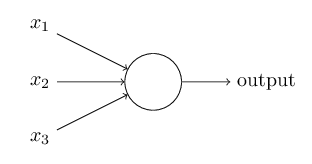
\includegraphics[scale=0.4]{figuras/capitulo-3/perceptron.png}
    \caption{A representation of the original McCulloch-Pitts perceptron. From~\cite{nielsenNeuralNetworksDeep2015}.}
    \label{fig:perceptron}
\end{figure}

The basic idea of NN is to mimic the way the brain works, and more specifically, the way 
neurons interact with each other. In the modern form of NN, this interaction is highly 
idealized in the sense that the actual human brain does not follow the same form of 
interaction, but it is somewhat a rough approximation. In 1947, Pitts and McCulloch~\cite{pittsHowWeKnow1947} devised the \emph{perceptron}, an idealized model of a neuron. This perceptron can be observed in \autoref{fig:perceptron}. Here, the middle circle is the perceptron or \emph{unit}, and it accepts three inputs \(x_1, x_2, x_3\), or equivalently \(\bm{x}=(x_1, x_2, x_3)\) with \(\bm{x}\) a \(3\)-dimensional input vector. The output of the McCulloch-Pitts perceptron is a single binary output, it can either return a \(0\) or a \(1\). Then, in 1958, Rosenblatt~\cite{rosenblattPerceptronProbabilisticModel1958} extended this idea and introduced a way to compute the output of the perceptron. He introduced what he called \emph{weights}, and gave a weight to each of the three inputs, \(w_1, w_2, w_3\). Later, he proposed to compute the output as a weighted sum of each of the three inputs, such that the output would have the following form,
\begin{equation}
    \text{output} = \begin{cases}
        0 \quad \text{if} \quad \sum_{i} w_i x_i \leq \varepsilon \\
        1 \quad \text{if} \quad \sum_{i} w_i x_i > \varepsilon
    \end{cases}
    \; ,
    \label{eq:output-perceptron}
\end{equation}
where \(\varepsilon\) is a \emph{threshold} value. This model is simple, yet effective. If 
one input would be more important than the other, the weight could be adjusted to reflect 
this. As simple as the model is, it is a good approximation of how decision-making models 
can be constructed efficiently. Furthermore, a more complex decision-making system can be built if several perceptrons are connected with each other. After all, the inputs and outputs of a single perceptron do not have limitations, and they can well be defined to be the inputs and outputs of other perceptrons as well. Instead of using a simple perceptron, a more complex structure can be built upon using several of them. If \emph{layers} of perceptrons are stacked between each other, a more complete model of decision-making is created. This is the case of the \emph{multilayer perceptron}, or MLP, shown in \autoref{fig:multi-perceptron}.

\begin{figure}
    \centering
    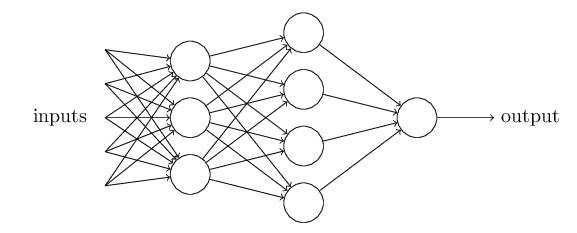
\includegraphics[scale=0.4]{figuras/capitulo-3/multi-perceptron}
    \caption{A representation of several perceptrons connected with each other. From~\cite{nielsenNeuralNetworksDeep2015}.}
    \label{fig:multi-perceptron}
\end{figure}

Despite this, the model has serious drawbacks. For one, 
there is no clear understanding of the threshold value and what it is. On the other hand, 
having the perceptron output just two values might make it inaccessible in the most general 
case. After all, the idea of NN is to learn a mapping, a function that in general is 
real-valued. Finally, how are the weights adjusted? Are these values picked randomly? Does 
the user choose them? If in fact NN are learning models, then there is no real reason why 
the user would likely pick the weights for each problem they need to solve. All of this 
questions will be addressed in a later section, when training is discussed in more detail.
For now, architectures and activations functions will be presented next. These topics will
provide answers as to how the output of perceptrons can be modified to return other values,
rather than just a \(0\) or \(1\).

\subsection{Architectures and Activation Functions}
Now that a complete network of perceptrons has been defined, it is time to discuss one 
important issue with them. First, it might be easier to deal with a different notation 
than just using threshold values. It is simpler to use the language of Linear Algebra 
and define the output expression shown in \autoref{eq:output-perceptron} using the dot product as follows,
\begin{equation}
    \text{output} = \begin{cases}
        0 \quad \text{if} \quad \bm{w} \cdot \bm{x} + b \leq 0 \\
        1 \quad \text{if} \quad \bm{w} \cdot \bm{x} + b > 0
    \end{cases}
    \, ,
    \label{eq:output-dot}
\end{equation}
where \(\bm{c} \cdot \bm{d} = \sum_{i}^{N} c_i \, d_i\) is the dot product between 
the $N$-dimensional vectors \(\bm{c}\) and \(\bm{d}\). Now, there is a new value, 
called the \emph{bias} term, defined as \(b\) in \autoref{eq:output-dot}. This new term is 
the value that is added to each perceptron and it can be interpreted as a measure of how 
easy it is to get the perceptron to output \(1\).

\begin{figure}
    \centering
    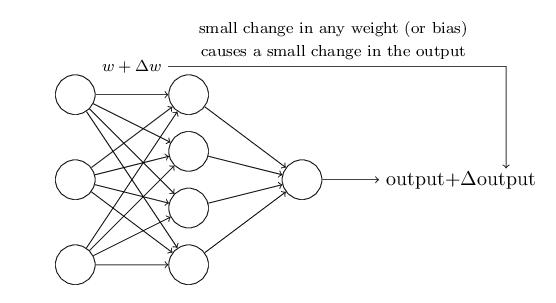
\includegraphics[scale=0.4]{figuras/capitulo-3/learning-weights}
    \caption{Visualization of the basic training mechanism in a neural network. By inducing a small change to the weights, a small change in the output is expected. From~\cite{nielsenNeuralNetworksDeep2015}.}
    \label{fig:learning-weights}
\end{figure}

There is now the following issue to address, and that is that the output is only \(0\) or 
\(1\). The issue here is that NN are expected to learn complex mappings between inputs and 
outputs, and if the weights are adjusted a minimal amount, for instance a value of 
\(\Delta w\), then the output should change just a small amount, proportional to the change 
in the weights. However, if the output is either a \(0\) or \(1\), then a small change will 
trigger a drastic change, and learning will not be entirely possible. A representation 
of this idea can be seen clearly in \autoref{fig:learning-weights}. The pertaining question 
here is, is there a way to change this behavior? The answer is yes, but to do so, a new 
type of perceptron, as well as a NN \emph{architecture} must be introduced.

The \emph{sigmoid} perceptron is a modification to the McCulloch-Pitts original perceptron which can provide a continuous value to the output by using a continuous function. This function, the \emph{sigmoid} function, is defined as
\begin{equation}
    \sigma(z) \coloneqq \frac{1}{1 + \exp{\left( -z \right)}}
    \; .
    \label{eq:sigmoid}
\end{equation}
Instead of the output being just \(0\) or \(1\), \autoref{eq:output-dot} is now replaced by the following equation, using now \autoref{eq:sigmoid},
\begin{equation}
    \text{output} = \frac{1}{1 + \exp{\left(- \sum_{i} w_i x_i + b\right)}}
    \; .
    \label{eq:output-sigmoid}
\end{equation}
This function might seem to drastically change the behavior and original intention of the 
McCulloch-Pitts perceptron. However, in reality, the sigmoid function is just a smoothed 
version of the original perceptron. With this modification, when a small change is done in 
the weights of the network, a small change will be expected in the output. The amount of 
change, and how this change happens, will be discussed in the next section when training is presented.

If different functions are used instead of the sigmoid function, the network is expected to 
behave differently with each one. The choice of the function is so important, that not only 
have these function taken in a particular name\textemdash \emph{activation functions}\textemdash, but there has been extensive research in this area~\cite{chenUniversalApproximationNonlinear1995,nwankpaActivationFunctionsComparison2018,agostinelliLearningActivationFunctions2015,ramachandranSearchingActivationFunctions2017}. 
In practice, the choice of activation function can make a NN perform better in 
certain classification tasks, e.g. object recognition, segmentation, and others; as well as 
in regression tasks. Activation functions can also help the NN perform faster, which is 
an important aspect of the training mechanisms and practicalities of
NN~\cite{fengPerformanceAnalysisVarious2019,biswasTanhSoftDynamicTrainable2021}.

Finally, it is important to mention that the \emph{topology}, or \emph{architecture}, of 
the network has been subject to significant research in recent times. For instance, if more 
layers are added in between layers, the NN takes in a different name, a \emph{deep neural network}. Deep neural networks have been the quintessential model of the revolutionary and 
extremely popular field of \emph{deep learning}~\cite{goodfellowDeepLearning2016}. In deep 
learning, NN architectures are extended to be larger, deeper, and more complex than simple 
multi-layer perceptrons. These new models can be thought of being several multi-layer 
perceptrons, each stacked upon each other.
Furthermore, deep learning attempts to generalize the simple perceptron model and introduce 
better models that can perform with greater accuracy in certain tasks. The explosion of 
deep learning came when \emph{convolutional neural networks} were applied successfully in 
the AlexNet architecture~\cite{krizhevskyImageNetClassificationDeep2012}. There other kinds 
of important variations in the topology of the network, such as the U-shaped networks use 
for medical image segmentation~\cite{ronnebergerUNetConvolutionalNetworks2015}; V-shaped 
networks used for remote sensing~\cite{abdollahiVNetEndtoEndFully2020}; and very deep 
topologies that can track images in real time~\cite{redmonYOLOv3IncrementalImprovement2018}.

\subsection{Training}
Choosing the correct activation function and the appropriate topology is hard, and a lot of 
experimentation is needed. But even if these could be chosen automatically, there is still 
a latent issue here: how weights can be adjusted. Up until this section, this issue has 
been left aside and it is now time to address it. To do so, it is imperative to remember 
the sole purpose of NN and ML methods for classification and regression tasks: 
\emph{to learn a mapping or function}. 
Assuming it is possible to have a training set \(\mathcal{D}\) with enough examples, 
containing both inputs and outputs, the function that determines the relationship between 
them can be learned by a NN. In general, this is referred to as the 
\emph{universal approximation theorem}, which shall be the topic of the next section.

The topic for this section is to answer the question of how this learning is carried out in 
the first place. And to do so, it is useful to recall the information from 
\autoref{fig:learning-weights} in that, if the weights are modified then the output is 
expected to change. Now, there are several questions that need an answer in that figure. 
For instance, what is the proportion between the change in the weights to the change in the 
output? If the weights are changed by half, is the output expected to change in the same 
amount? For the case of classification, there are only categorical outputs, so how are 
changes to the weights passed on the output? It seems that there needs to be a quantity 
that must inform the \emph{learning} mechanism how much should the weights change in order 
to get the correct output from the network. 

In order to address those questions, there needs to be a relationship between the output, the weights and the bias. Fortunately enough, calculus provides such information in the 
following way,
\begin{equation}
    \Delta \ \text{output} \ \approx \sum_{j} \left[ \frac{\partial \ \text{output}}{\partial w_j} \Delta w_j \right] + \frac{\partial \ \text{output}}{\partial b} \Delta b
    \; ,
    \label{eq:output-combination}
\end{equation}
where the sum is over all the weights in the network, \(w_j\), and \(\partial \ \text{output} \, / \, \partial w_j\) and \(\partial \ \text{output} \, / \, \partial b\) denote 
the partial derivatives of the output with respect to the weights and bias, respectively. 
In other words, these derivatives represent \emph{by how much} the output changes if the 
weights and bias are modified. Yet, there is still even more information from \autoref{eq:output-combination} 
that is extremely useful. If looked at closely, \autoref{eq:output-combination} actually 
represents a \emph{linear combination} of terms that, together, form the change to the 
output. This means that both, the weights and the bias, must contribute to the change in 
the output, and the amount is provided by the partial derivatives. So with just this much, 
the answer to the question of \emph{how much} is now answered. But now there is the burning 
question of how to compute the partial derivatives. Well, this question is easy to answer, 
because assuming that the NN is using sigmoid neurons, then the derivative can be reduced 
to the following expression,
\begin{equation}
    \frac{d}{dz} \sigma (z) = \sigma^{\prime} (z) = \frac{1}{1 + e^{-z}}  \cdot \left(1 - \frac{1}{1 + e^{-z}}\right) = \sigma (z) \, \left(1 - \sigma (z)\right)
    \; ,
    \label{eq:dsigmoid}
\end{equation}
where some steps were skipped to avoid taking too much space. Recalling that the output from 
the sigmoid perceptron is given by \autoref{eq:output-sigmoid}, together with \autoref{eq:dsigmoid}, 
the partial derivatives from \autoref{eq:output-combination} can be obtained without much
effort. In more general cases when the perceptron uses a different activation function than 
the sigmoid, the computation of derivatives is carried out using modern tooling known as 
\emph{automatic differentiation}~\cite{baydinAutomaticDifferentiationMachine2018}.

Now, the issue of addressing how the learning mechanism is informed can be solved by 
introducing the \emph{cost function}. The cost function, also referred to sometimes as 
\emph{loss} or \emph{objective}, is a function that measures how the NN is approximating 
the underlying function. This is, in fact, the same concept as the performance measures 
encountered in \autoref{sec:performance}. In fact, cost functions are metrics that address 
how good the approximation of the NN is. And so this issue has also been addressed. 
However, how is this cost function, and \autoref{eq:output-combination} used to make the NN 
learn the mapping? For this, we turn to optimization and the powerful method of \emph{gradient descent}. To help illustrate the learning mechanism, the mean squared error in 
\autoref{eq:mse} will be used. However, this is not the only metric that can be used, and 
in fact several research advancements have been carried out in this direction~\cite{fontenla-romeroNewConvexObjective2010,liDiversityPromotingObjectiveFunction2016}.

Numerical optimization is a rigorous mathematical subject, and the use of gradient descent techniques can not be summarized in this section. For that, the great book by Nocedal and Wright is an excellent reference for this topic~\cite{nocedalNumericalOptimization2006}.
Here, only the main results will be mentioned and used. In optimization, specifically \emph{unconstrained optimization}, the task is to find the value of an input vector \(\bm{x}\) that \emph{minimizes the function} \(f\), such that \(f(\bm{x}) = 0\). The fact that it is unconstrained is because there is no restriction in the bounds of \(\bm{x}\), or in the form of \(f\), which in general is a non-linear function. In the context of optimization, \(f\) is referred to as a cost function, or objective function.
Now, a relation between optimization and NN can be made by noting the following fact. The 
purpose of NN is to learn the function that relates inputs and outputs in a given data set. 
Or in the context of optimization: \emph{to minimize the error between the true values and 
the approximation values}. The \emph{true values} correspond to the outputs in the data 
set, and the \emph{approximation values} to the outputs from the NN. So, in essence, the 
task is to find the best weights \(w_j\), and the best bias \(b\), that minimize the 
following cost function,
\begin{equation}
    C(\bm{w}, b) = \frac{1}{2 N} \sum_{i=1}^{N} { \left[y_i - \hat{y}_{i}(\bm{w}, b) \right] }^2
    \; .
    \label{eq:cost-nn}
\end{equation}
Here the sum goes over all $N$ training samples in the training data set, and the output 
from the NN \(\hat{y}_{i}(\bm{w}, b)\) depends on the values of the weights
\(\bm{w}\) and bias \(b\).

There is now one step left for the training procedure to be completely characterized, and 
that is to define a way to \emph{update} the weights and bias accordingly so that 
\autoref{eq:cost-nn} is minimized. For this purpose, \emph{gradient descent} is used. 
Gradient descent is an iterative optimization method based on first-order derivative 
information. The idea is to use the information from the gradient of the objective function 
to drive the minimization to minimum, which in general corresponds to a \emph{local minimum}. The derivation of the method is left for a specialized reference on the 
matter~\cite{nocedalNumericalOptimization2006}, and the main results will be used here. In 
the context of NN, the idea to update the weights and bias so as to minimize the cost 
function. Thus, the gradient descent method is introduced, which follows the expression,
\begin{equation}
    \begin{aligned}
        \bm{w}_{j+1} &= \bm{w}_{j} - \eta \frac{\partial C}{\partial \bm{w}_{j}} \\
        b_{j+1} &= b_{j} - \eta \frac{\partial C}{\partial b}
    \end{aligned}
    \label{eq:gradient-descent-nn}
\end{equation}
where the index \(j\) represents each of the steps taken to update each value. These steps 
are also sometimes referred to as iterations. Hopefully, by doing several updates of 
\autoref{eq:gradient-descent-nn}, then \autoref{eq:cost-nn} can be minimized and the 
appropriate value of the weights and bias would have been found.

In practice, this simple rule is not actually followed for one simple reason. If looked at 
closely, \autoref{eq:gradient-descent-nn} actually takes in all the information gathered so 
far, and this includes the training examples, which are encoded in the cost function. But 
if the data set contains thousands of examples, then the optimization can not be carried 
out due to current limitations in modern hardware. So a simple modification is used, where 
instead of choosing all the training examples at once, a small sub-set is chosen randomly 
and then the gradient descent is used on this sub-set. 
This procedure is repeated until all the 
training examples have been selected. This is referred to as a 
\emph{pass}. At the end of this pass, all the obtained values are averaged, and this 
average is used to update the weights and bias. This can be repeated for as many 
\emph{passes} as needed, or wanted. This simple modification is the actual 
method use, and goes by very popular name of \emph{stochastic gradient descent}.
Extensive research has been conducted in this area as well, from introducing simple
accelerating terms to the gradient descent rule. For instance, the Nesterov momentum 
gradient descent method~\cite{ruderOverviewGradientDescent2017}, or the Adam 
method~\cite{kingmaAdamMethodStochastic2017}, which is in fact the method used in this work 
and will be presented at a later part.

To summarize, the training mechanism of NN is as follows. Assuming a training data set 
\(\mathcal{D}\) is available, then a cost function is chosen. In practice, the most common 
has the form of \autoref{eq:cost-nn} but it can be any other. Then, the weights and biases 
are initialized at random. After that, the main loop of the algorithm is to repeat the 
steps shown in \autoref{eq:gradient-descent-nn} while keeping track of the minimum. When a 
certain minimum has been achieved, a performance measure can be used to check whether the NN 
has a good performance for the task given. This concludes, roughly speaking, the common 
practice of modern ML.

\subsection{Universal Approximation Theorem} \label{sec:approximation-thm}
To close this section on ML and NN, an overly important fact of NN must be stated. Before, 
it was mentioned that the goal of tasks such as classification and regression is for the 
model to learn or approximate the function that maps the input to the output for a given 
data set. For this reason, NN were presented, along with their learning mechanism. However, 
what \emph{guarantee} is there that NN \emph{will} approximate the function? Further, 
\emph{can NN, in fact, approximate a function}? In a previous section, it was briefly 
mentioned that NN can in fact \emph{learn} any function, and that will be the topic of this 
section.

Indeed, just as mentioned before in the section for Approximation Theory, there exists a 
similar result for NN. This result, which are actually a series of results, come from the 
mathematical research of NN. The results are known altogether as the \emph{universal 
approximation theorem}. To really understand these results, advanced mathematical results 
should be employed. However, there is no need to extend the current section to such 
lengths. Instead, following the research from Hornik and Cybenko~\cite{hornikMultilayerFeedforwardNetworks1989, hornikApproximationCapabilitiesMultilayer1991, cybenkoApproximationSuperpositionsSigmoidal1989}, 
the main results will be stated here to be interpreted.

\begin{figure}
    \centering
    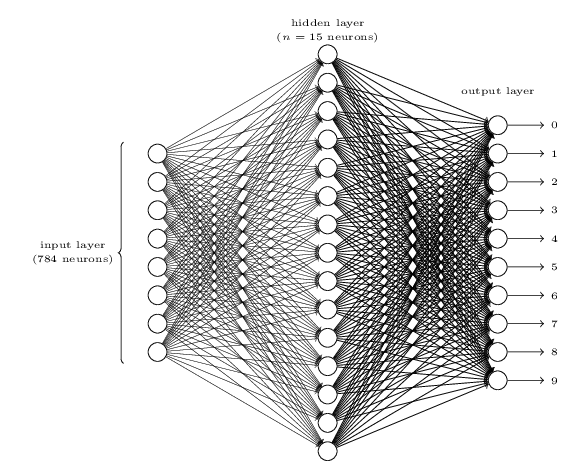
\includegraphics[scale=0.4]{figuras/capitulo-3/tres-capas.png}
    \caption{A multi-layer perceptron with three layers: the first layer is the \emph{input layer}; the middle layer is known as the \emph{hidden layer}; and the last layer is known as the \emph{output layer}. From~\cite{nielsenNeuralNetworksDeep2015}.}
    \label{fig:hidden-layer}
\end{figure}

In short, Hornik and Cybenko showed that, given the sigmoid function and a given topology, 
there exists an arbitrary number of nodes that are needed to \emph{approximate} any 
\emph{continuous} function. The topology is a three layer topology, similar to the one in 
\autoref{fig:hidden-layer}, where there is an input, a hidden and an output layers. This 
results is also similar to \autoref{approx}; however, in this case there is no polynomial 
but a NN instead. The arguments that follow this result is beyond the scope of this work, 
but the result remains valid. Then, as the research for the mathematical framework of NN 
advanced, newer results have seen the light that extend these results even more. Now, there 
is a clear understanding that not only the sigmoid function can be used, but any non-affine 
continuous function that it continuously differentiable~\cite{parkMinimumWidthUniversal2020}. Furthermore, there is also no need to restrict the case to just width, but also depth, 
from which the generalization to deep learning 
follows~\cite{zhouUniversalityDeepConvolutional2020,bernerModernMathematicsDeep2021}.
In this work, these guidelines are used to create simple topologies for NN that can 
actually satisfy the conditions of the theorem. A topology similar to 
\autoref{fig:hidden-layer} with a large amount of nodes for each layer, which should 
suffice to satisfy the conditions of the theorem. However, in practice, it has been shown 
that \emph{overparametrization}\textemdash when there are way more weights and bias to adjust than needed \textemdash is the key to generalization in 
NN~\cite{neyshaburRoleOverparametrizationGeneralization2018,cohenLearningCurvesOverparametrized2021}.
This means that most of the time, the common practice is to just use deep topologies, which 
mean a large number of layers and a large number of nodes for each layer, and use this 
overparametrization to leverage the generalization that this provides. So, in a sense, one 
might say that the universal approximation theorem is always satisfied in modern ML practice.

\section{Evolutionary Computation}
In this section, Evolutionary Computation (EC) is presented and discussed. Much like the 
driving force of perceptron is to mimic the brain and its intelligence, the inspiration 
behind EC is the way nature adapts itself through 
evolution~\cite{fogelWhatEvolutionaryComputation2000}. Although, in reality, evolution 
takes millions of years but it eventually creates variations that adapt and \emph{converge} 
to a particular goal. This particular goal, as described by Darwin, is to be fit to its 
surroundings and survive. The idea behind EC is to use this powerful mechanism of evolution 
and apply it to complex problems, with the use of modern computational and mathematical 
resources to facilitate and empower a simplified version of evolution. In the most general 
case, evolution is roughly a two-step process: first comes \emph{variation} and then comes 
\emph{selection}. Algorithms based of EC use these properties and, depending on how these 
variations and selections occur, the algorithms are named and used differently. In 
particular, for this work the focus will be \emph{evolution strategies}, which will be 
address in a later section. However, there is also \emph{genetic algorithms}, 
\emph{evolutionary algorithms}, and other~\cite{kacprzykSpringerHandbookComputational2015}.

\begin{figure}
    \centering
    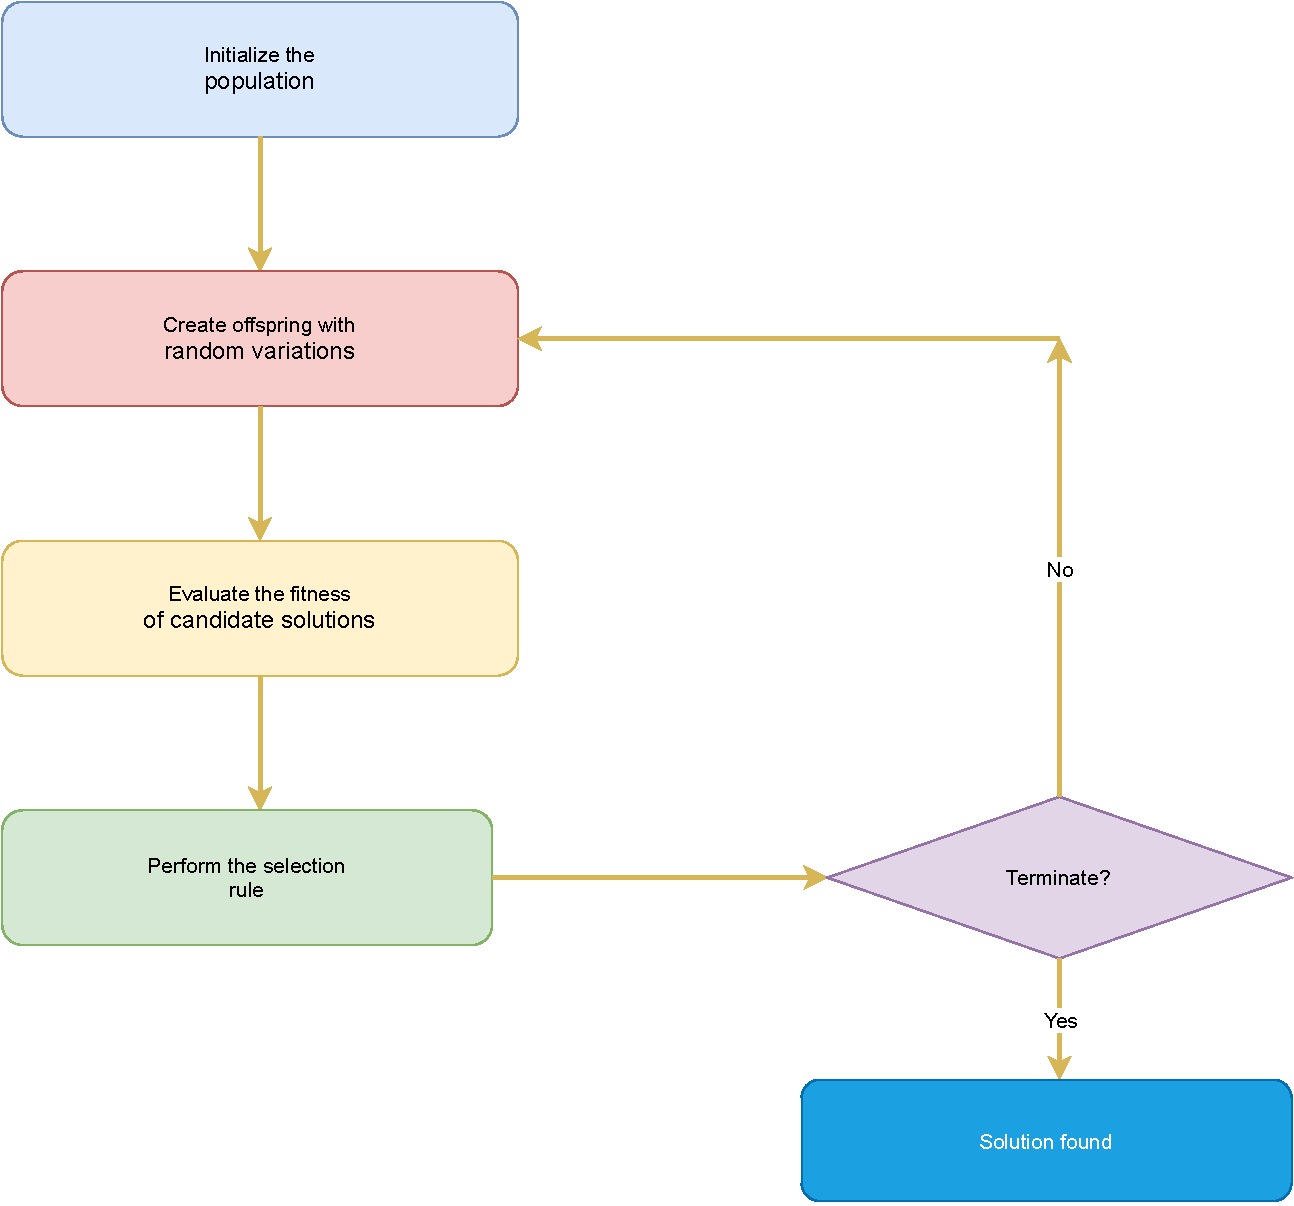
\includegraphics[scale=0.67]{figuras/capitulo-3/evolutionary-optimization.pdf}
    \caption{Evolutionary algorithms always start by creating a population of solutions. New solutions are then created by varying those from the original population. Then, the solutions are measured with respect to how well they address the task. Finally, a selection criterion is applied extract the best solutions so far. The process is iterated using the selected set of solutions until a specific criterion is met.}
    \label{fig:evolutionary-optimization}
\end{figure}

As mentioned before, there is a common procedure in evolution, and this has been translated 
to computer science and its application in EC. The basic procedure is as follows: for a 
given problem, an initial population of possible \emph{solution} is created; then, those 
solutions that are \emph{fit} or \emph{approximate} the solution are kept, those that not 
are discarded; finally, the successful candidate are mixed, creating offsprings with 
\emph{variations} of all the other possible solutions. With these steps, a common EC 
algorithm can be constructed, and in general this is case. The advantage of using EC is 
that of \emph{adaptability}. Many of these algorithms are suited for hard problems, some of 
which are impossible to solve with traditional methods, or at least take a long time to 
find a solution, such as the famous traveling salesman 
problem~\cite{dorigoAntColonySystem1997}. Flexibility, adaptability and generalization are 
the advantages of EC algorithms. When used in the popular StarCraft computer videogame, the 
AlphaStar system~\cite{arulkumaranAlphaStarEvolutionaryComputation2019} performed 
surprisingly better than the top players in the world.

However, the lack the general ease of use in some cases, as well as the difficulty to 
implement them might be troublesome in some other cases. Also, EC algorithms tend to have 
many parameters to adjust. For instance the total number of solutions in the population, 
the number of offsprings, and so on. In the case of EC algorithms, there is no \emph{one 
size fits all}, so this can make them hard to deal with. In the present work, EC algorithms 
will be used for non-linear unconstrained optimization, and in particular, in the sub-field 
of \emph{derivative-free optimization}. This will be discussed in the next section.

EC algorithms have been used for optimization in cases where the objective function is not 
\emph{smooth}, does not posses a \emph{continuous derivative}, or when it is too 
\emph{costly} to search for a solution in finite 
time~\cite{kacprzykSpringerHandbookComputational2015}. The basic functionality of EC 
algorithms for optimization follow the diagram from 
\autoref{fig:evolutionary-optimization}. With EC algorithms, the idea is to form an initial 
population of solutions, then to vary those solutions while keeping track of the fitness of 
the objective function. By varying the possible solutions, it is expected that these will 
\emph{follow an evolutionary process}, and eventually reach a minimum. In particular, EC 
algorithms are best suited for \emph{global optimization}, which is the search for minima 
in a large search space, without reaching any local minima along the way. The purpose 
behind this is to \emph{explore} the search space and look for the values that best 
minimize the function. After all, EC algorithms are \emph{approximation algorithms}, i.e. 
this methods do not attempt to find the best solutions, but to 
\emph{find a possible solution} to the problem.

\subsection{Derivative-free and Black-box Optimization}
In optimization tasks, the best algorithms are those that include some kind of information 
about \emph{derivatives}. For instance, the Newton method, and Newton-like methods such as 
BFGS~\cite{nocedalNumericalOptimization2006}, are some of the best for their speed, 
accuracy and convergence properties. Mathematically rigorous frameworks can be used to 
understand these algorithms, and can also be used to understand their convergence 
properties. Another similar optimization method was encountered before, the gradient 
descent method, which by leveraging the gradient information of the objective function a 
local minimum could be found by iterative steps.

However, the derivative information is not always available. When such cases are 
encountered, the only methods capable of providing solutions are known as 
\emph{derivative-free} methods. These methods try to search the best solution, using 
different kinds of strategies, such as the 
trust-region~\cite{byrdTrustRegionAlgorithm1987}, quadratic polynomial 
approximation~\cite{powellUOBYQAUnconstrainedOptimization2002}, and the most recent and 
interesting approach is that of surrogate model 
optimization~\cite{forresterRecentAdvancesSurrogatebased2009}. In each case, the objective 
function is approximated using some form of interpolation, or surrogate model, and the 
original search space is projected onto a new search space where the approximation can be 
optimized efficiently. With this approach, derivatives are no longer needed and 
optimization can be performed, but not without its drawbacks. First and foremost, the 
method relies entirely on function evaluations. If the function is \emph{costly} to 
evaluate, then this methods will take a long time to find a suitable solution. Further, the 
search space will be explored, and this can considerably slow down the optimization 
procedure. After all, these methods try to explore and map the whole search space, but if 
the search space is quite large, the optimization procedure will suffer greatly in terms of 
performance. Finally, the \emph{no free lunch} theorem states that, averaged over all 
optimization problems, all optimization methods perform equally 
well~\cite{adamNoFreeLunch2019}. This means that if a particular derivative-free method is 
not providing sufficiently good results, then there must exist another optimization method 
that should give sufficiently good solutions. In other words, several algorithms must be 
tested against each other, given that there are enough computational resources to do so.

As mentioned before, sometimes there is not derivative information about the objective 
function, but more than that, objective function evaluations are \emph{costly}. This means 
that, for a given input \(\bm{x}\) and an objective function \(f \colon \mathbb{R}^n \mapsto \mathbb{R}\), the evaluation \(f(\bm{x})\) will take a long time. Further, in 
most cases when this is true, the \emph{analytical or functional form} of the objective 
function \emph{is not known}. When a particular objective function satisfies these 
conditions, it is referred to as a \emph{black-box function}. When optimizing costly 
black-box function, the main goal is to \emph{minimize} the number of evaluations of the 
function. This is done by sampling the search space \emph{intelligently} so as to not 
evaluate the objective function where there is no sign of a minimum.

Black-box functions can, in general, be any type of function, either mathematical or 
computational. When the function is computational, this can represent code that performs 
several tasks, each of which might take a considerable amount of time and computing 
resources. In such cases, black-box optimization algorithms are the key to solving the 
problem. Or maybe the black-box function is not too costly, but instead the true form of 
the function is not known. Again, black-box optimization algorithms are the best choice
in that scenario. In the next section, a particular black-box optimization algorithm 
derived from EC methods will be reviewed and presented, which will be extensively used in 
chapter 5 of this thesis.

\subsection{Natural Evolution Strategies}
One algorithm that stands out for its robustness and flexibility in dealing with black-box 
optimization tasks is the \emph{natural evolution strategy} algorithm (NES), presented in 
2014 by Wierstra \emph{et al}~\cite{wierstraNaturalEvolutionStrategies2014a}. This 
algorithm is a derivative of the Evolution Strategies (ES) family of algorithms, which 
follow closely the principles of EC. In ES algorithms, the principal characteristics are 
the ease of dealing with high-dimensional optimization problems, and low number of function 
evaluations. Also, unlike other EC algorithms, ES methods evaluate the fitness of the 
functions in batch instead of individually, allowing for more efficient computation and 
solution space search in general. The most prominent algorithm in the ES family of methods 
is the CMA-ES, or Covariance Matrix Adaptation-Evolution 
Strategy~\cite{hansenCMAEvolutionStrategy2006}.
In general, ES methods do two main things. To perform \emph{variation}, multivariate normal 
random vectors are used. To perform \emph{mutation}, these algorithms modify different 
aspects of such multivariate normal distribution. The case of CMA-ES is to modify and adapt 
the covariance matrix in order to perform better at each step.

However, the method of NES is different. Instead of modifying the covariance directly, the 
information on the \emph{natural gradient} is exploited. To understand this method more 
clearly, let \(f \colon M \subseteq \mathbb{R}^n \mapsto \mathbb{R}\) be a black-box 
function, and the problem of optimization is to search for a vector \(f(\hat{x}) \in M\) 
such that a \emph{local minimum} is found, where the local minimum is defined as,
\begin{equation}
    \exists \; \epsilon > 0 \quad \forall x \in M \; \colon \; 
    \lVert x - \hat{x} \rVert < \epsilon \Rightarrow f(\hat{x}) \leq f(x)
    \: .
    \label{eq:local-minimizer}
\end{equation}
Now, the goal is not to minimize the objective function directly, but to minimize an \emph{expected fitness} under a particular search distribution. This means that the parameters searched will define a continuous probability distribution. This cost function is now expressed as,
\begin{equation}
    J(\theta) = \mathcal{E}_{\theta} \left[ f(\bm{x}) \right] = 
    \int f(\bm{x}) \, \pi (\bm{x} \, \vert \, \theta) \, d \bm{x}
    \; ,
    \label{eq:expected-fitness}
\end{equation}
and using this cost function, together with a gradient descent-like rule, the purpose of NES is to find the best 
\emph{probability distribution} that will eventually be sampled to obtain a minimizer for 
the original objective function. In other words, the NES method is not looking for the 
minimizer itself in a search space, but it is looking for the probability distribution 
that, when sampled, will give in average the minimizer for a particular local minimum of 
the objective function.

Still, the gradient information is unknown, as well as the true form of the search distribution, \(\pi (\bm{x} \, \vert \, \theta)\). But it is also impossible to obtain a gradient estimation without explicit information about the probability distribution. Here is where the NES provides a novel way of dealing with this problem. First, the search distribution is fixed to be a multivariate normal distribution,
\begin{equation}
    \pi (\bm{x} \, \vert \, \theta) = 
    \frac{1}{{(2 \pi)}^{d/2} \text{det} \; \bm{\Sigma} } 
    \cdot
    \exp{\left(- \frac{1}{2} {\left(\bm{x} - \bm{\mu}\right)}^{\top}
    \bm{\Sigma}
    \left(\bm{x} - \bm{\mu}\right) \right)}
    \; ,
    \label{eq:multivariate-gaussian}
\end{equation}
with \(\bm{\Sigma} \in \mathbb{R}^{d \times d}\) the covariance matrix and 
\(\bm{\mu} \in \mathbb{R}^{d}\) 
the mean vector of a multivariate normal distribution. The parametrization 
\(\theta \coloneqq \left\langle \bm{\mu}, \bm{\Sigma} \right\rangle\) is the link between 
these probability distributions. With this information, the gradient is obtained with some important mathematical manipulations, which is approximately,
\begin{equation}
    \nabla_{\theta} J(\theta) \approx \frac{1}{\lambda} \sum_{i=1}^{\lambda}
    f(x_k) \, \nabla_{\theta} \log{\pi(x_k \, \vert \, \theta)}
    \; ,
    \label{eq:search-gradient}
\end{equation}
and it is also known as the \emph{search gradient}, and the gradient descent rule is just
\begin{equation*}
    \theta_{j + 1} = \theta_{j} + \eta \nabla_{\theta} J(\theta)
    \; .
\end{equation*}
The parameter \(\lambda\) in \autoref{eq:search-gradient} is the population size of the 
method, which in general is a small number, \(\lambda \approx 20 - 35\).

However, this is just the search gradient, and it has some serious disadvantages. One of 
which is the fact that the gradient descent update rule is not independent of the 
distribution, so the parameters can take different proportions. Another important aspect of 
the gradient descent rule is that it might be slow in terms of convergence for black-box 
objective functions. For this reason, the \emph{natural gradient}~\cite{amariNaturalGradientWorks1998,amariWhyNaturalGradient1998} is introduced, which 
modifies the gradient descent rule to be,
\begin{equation}
    \theta_{j + 1} = \theta_{j} + \eta \cdot \bm{F}^{-1} \nabla_{\theta} J(\theta)
    \; .
    \label{eq:natural-gradient}
\end{equation}
Here, \(\bm{F}\) is the \emph{Fisher information matrix} defined as,
\begin{equation}
    \bm{F} = \int \pi(\bm{z} \, \vert \, \theta) \; 
    \nabla_{\theta} \log{\pi(\bm{z} \, \vert \, \theta)} \;
    {\nabla_{\theta} \log{\pi(\bm{z} \, \vert \, \theta)}}^{\top} \;
    d \bm{z}
    \: ,
    \label{eq:fisher-matrix}
\end{equation}
but in practice it is estimated as,
\begin{equation}
    \bm{F} \approx \frac{1}{\lambda} \sum_{k=1}^{\lambda} 
    \nabla_{\theta} \log{\pi(x_k \, \vert \, \theta)} \;
    {\nabla_{\theta} \log{\pi(x_k \, \vert \, \theta)}}^{\top}
    \; .
    \label{eq:fisher-estimation}
\end{equation}

In summary, NES attempts to estimate the search distribution using the natural gradient 
such that, when sampled, the search distribution will in average output the minimizer to 
the objective function. Here, most of the details have been omitted for the sake of 
brevity, but the original work~\cite{wierstraNaturalEvolutionStrategies2014a} provides all 
the information needed to implement the method. In this work, though, a variant of the NES 
method is used, the \emph{distance-weighted exponential} (DXNES)
NES~\cite{fukushimaProposalDistanceweightedExponential2011,nomuraDistanceweightedExponentialNatural2021}. 
This method is a variation on the way the natural gradient and Fisher information matrix 
are obtained, but the core of the method remains the same.